\chapter{Robot Models}\label{c:models}
\section{Direct Drive Horizontal Model}

\begin{figure}[hbt]
\centering
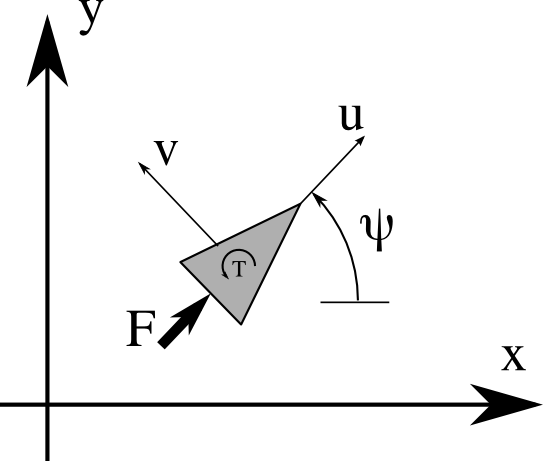
\includegraphics[width=\FigWidth\textwidth]{uni_model.png}
\caption{Illustration of the direct drive horizontal robot model.}
\label{f:uni_model}
\end{figure}

Three degrees of freedom.

\begin{itemize}
\item Model States
\begin{itemize}
\item $x$ and $y$: Position of the vehicle with respect to a fixed frame of reference.
\item $\psi$: Angular position of the vehicle relative to the $x$ axis.
\item $u$: Forward velocity of the vehicle with respect to the body-frame.
\item $v$: Lateral velocity of the vehicle with respect to the body-frame.
\item $r$: Angular velocity of the vehicle.
\end{itemize}
\item Inputs
\begin{itemize}
\item $F$: Force input in the foward direction with respect to the body-frame.
\item $T$: Torque input in the counter-clockwise direction.
\end{itemize}
\item Model Parameters
\begin{itemize}
\item $M$: Tranlational intertia (mass) of the vehicle
\item $I$: Rotational inertia (moment-of-inertia) of the vehicle
\item $d_u$: Tranlational damping/drag on the vehicle in the forward ($u$) direction
\item $d_v$: Tranlational damping/drag on the vehicle in the lateral ($v$) direction
\item $d_r$: 
\end{itemize}
\end{itemize}

Kinematics

\begin{eqnarray}
\dot{x} & = & \cos{(\psi)}u - \sin{(\psi)}v \\
\dot{y} & = & \sin{(\psi)}u + \cos{(\psi)}v \\
\dot{\psi} & = & r
\end{eqnarray}

Kinetics
\begin{eqnarray}
\dot{u} & = & -\frac{d_u}{M}u + \frac{1}{M}F \\
\dot{v} & = & -\frac{d_v}{M}v \\
\dot{r} & = & -\frac{d_r}{I}r + \frac{1}{I}T \\
\end{eqnarray}
If the damping factors ($d_u$, $d_v$ and $d_r$) are constants, this model represents linear drag behavior.
This chapter is about \gls{robotmodel}s.

\begin{ex}
Write a simulation - write the discrete-time formulation on paper first
\end{ex}

\begin{ex}
Test the simulation with some test inputs
\end{ex}

\begin{ex}
Choose a constant dt based on physical parameters
\end{ex}

\begin{ex}
Write the simulation using some linear algebra
\end{ex}

\
\begin{ex}
Write an open-loop  controller
Write a closed-loop controller
\end{ex}

\begin{ex}
Reformulate for differential drive
Figure~\ref{f:uni_model_diff}
\end{ex}

\begin{figure}[hbt]
\centering
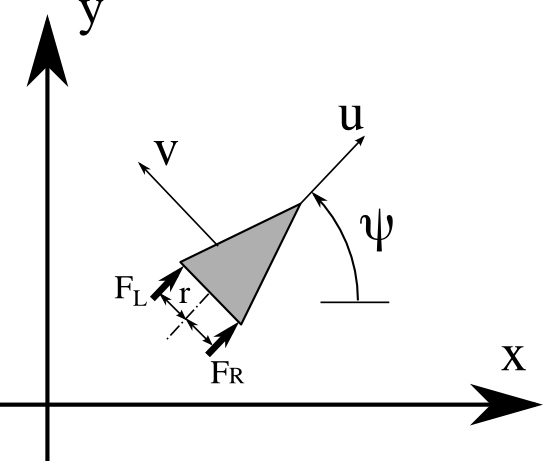
\includegraphics[width=\FigWidth\textwidth]{uni_model_diff.png}
\caption{Illustration of the differential drive variant of the horizontal robot model shown in Figure~\ref{f:uni_model}.}
\label{f:uni_model_diff}
\end{figure}
